\documentclass[conference]{IEEEtran}
\IEEEoverridecommandlockouts
% The preceding line is only needed to identify funding in the first footnote. If that is unneeded, please comment it out.
\usepackage{cite}
\usepackage{amsmath,amssymb,amsfonts}
\usepackage{algorithmic}
\usepackage{graphicx}
\usepackage{textcomp}
\usepackage{xcolor}
\usepackage{listings}
\usepackage{float}
\def\BibTeX{{\rm B\kern-.05em{\sc i\kern-.025em b}\kern-.08em
T\kern-.1667em\lower.7ex\hbox{E}\kern-.125emX}}
\begin{document}

\title{CSE 6603 - Data Management in the Cloud \\ Project Report \\ Improving efficiency of Microservices Autoscaling and Scheduling with Kernel Tracing}

\author{
    \IEEEauthorblockN{Samidhya Sarker}
    \IEEEauthorblockA{Roll: \textit{1018052049} \\ \textit{CSE, BUET}}
\and
    \IEEEauthorblockN{Md. Habibur Rahman}
    \IEEEauthorblockA{Roll: \textit{0422052014} \\ \textit{CSE, BUET}}
\and
    \IEEEauthorblockN{Dr. Muhammad Abdullah Adnan}
    \IEEEauthorblockA{Professor \\ \textit{CSE, BUET}}
}

\maketitle

\begin{abstract}
Designing distributed cloud applications that are decoupled into a bunch of small components (i.e. microservices) has been made easy with microservices architecture. One of the challenges in deploying microservices is finding the optimal amount of resources (i.e. size) and the number of instances (i.e. replicas) for each microservice so that you maintain good performance and don't waste resources or underutilize them. 
\end{abstract}

\begin{IEEEkeywords}
    cloud, linux, lttng, microservice, container
\end{IEEEkeywords}

\section{Introduction}
\subsection{Cloud Computing}
Hundreds of small, fine-grained components (referred to as "microservices") work together to serve end-user requests in a distributed environment under the microservices architecture, a recent and growingly popular paradigm for developing interactive and user-facing services\cite{netflix, azure, google, appEngine, burns}. There are various advantages to splitting up an application into smaller microservices. It enables several development teams to independently operate on disparate microservices that may be technologically dissimilar\cite{wolff}. Additionally, because each microservice may grow and operate independently based on its own state and incoming workload, the program as a whole performs better and is more reliable\cite{hao}. A microservices architecture may also make it easier to debug performance and accuracy problems \cite{b54}

\begin{figure}[!h]
    \begin{center}
        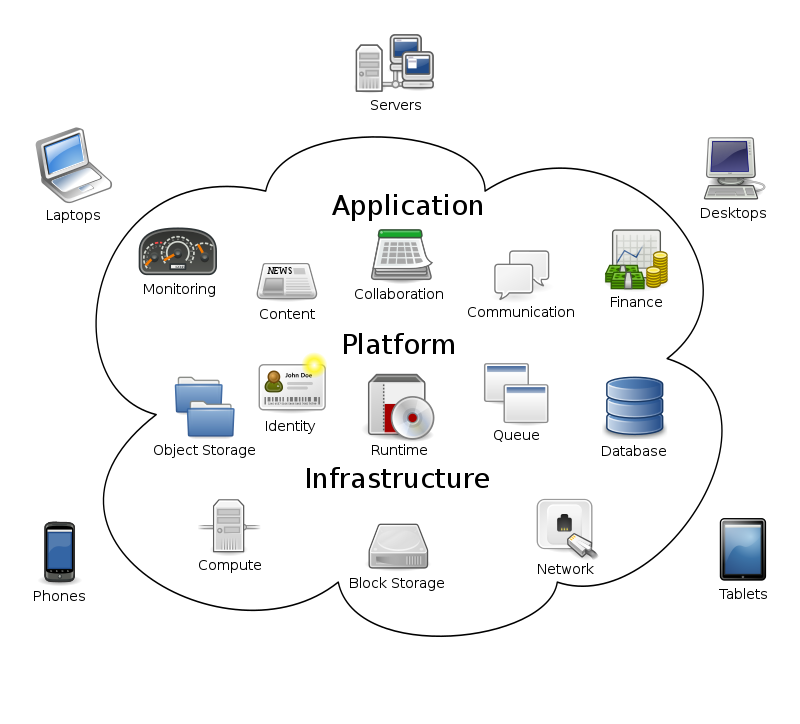
\includegraphics[width=0.4\textwidth]{figures/Cloud-computing.svg.png}
    \end{center}
    \caption{Cloud Computing}
    \label{fig:cloud}
\end{figure}


\subsection{Microservices}

Microservice architecture is an architectural pattern that arranges an application as a collection of loosely-coupled, fine-grained services, communicating through lightweight protocols. It allows teams to develop and deploy their services independently of others. Microservices are a popular architectural style for building applications that are resilient, highly scalable, independently deployable, and able to evolve quickly.

Interfaces need to be designed carefully and treated as a public API.

One technique that is used is having multiple interfaces on the same service, or multiple versions of the same service, so as to not disrupt existing users of the code. \cite{b3}

Decomposing an application into different smaller services can provide several benefits, such as modularity, scalability, integration of heterogeneous and legacy systems, and continuous integration, continuous delivery and deployment.

A successful microservices architecture requires a different approach to designing and building applications.
A microservices architecture consists of a collection of small, autonomous services.

Each service is self-contained and should implement a single business capability within a bounded context.

A bounded context is a natural division within a business and provides an explicit boundary within which a domain model exists.

\begin{figure}[!h]
    \begin{center}
        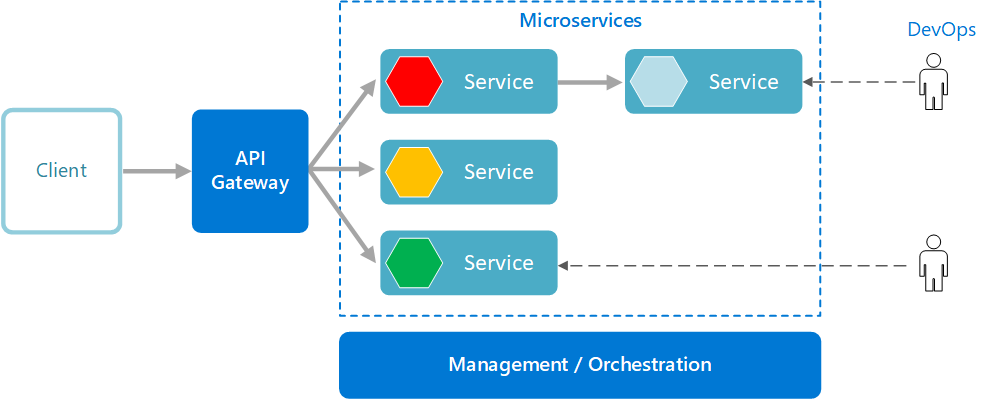
\includegraphics[width=0.4\textwidth]{figures/microservices-logical.png}
    \end{center}
    \caption{Microservice architecture}
    \label{fig:microservice}
\end{figure}

\subsubsection{Comaprison with monolithic architecture}

Microservices architecture splits up an application into independent codebases that perform one specific task. These modules communicate with each other through an Application Programming Interface to create the full functionality of an application.
Microservices allow an application to grow by being self-contained and managed by a team dedicated to that functionality.
Easy to scale: Using microservices, an application can be scaled horizontally, meaning each microservice can increase in size independently as its needs change.

Horizontal scaling can be less costly than vertical scaling, and there is no limit to how much an application can scale.
Microservices-based architecture allows teams to easily add additional functionality and new technologies to an application as needed. However, the way microservices are linked together adds a layer of complexity.
Requires specialized skills: Building a microservices architecture requires specialized knowledge which not all developers may have.

Teams who build microservices without the correct training can run into a myriad of challenges which may mean a delayed time to market and additional costs to bring in outside experts.
Distributed security and testing: Each module will have its own security vulnerabilities and bugs.

While this can be beneficial in preventing attacks, it also means more potential vulnerabilities to track, and debugging each individual element can become time-consuming.
Extra costs: Utilizing microservices may save some costs, but will also likely require additional development resources to manage each microservice and its dependencies.

\begin{figure}[!h]
    \begin{center}
        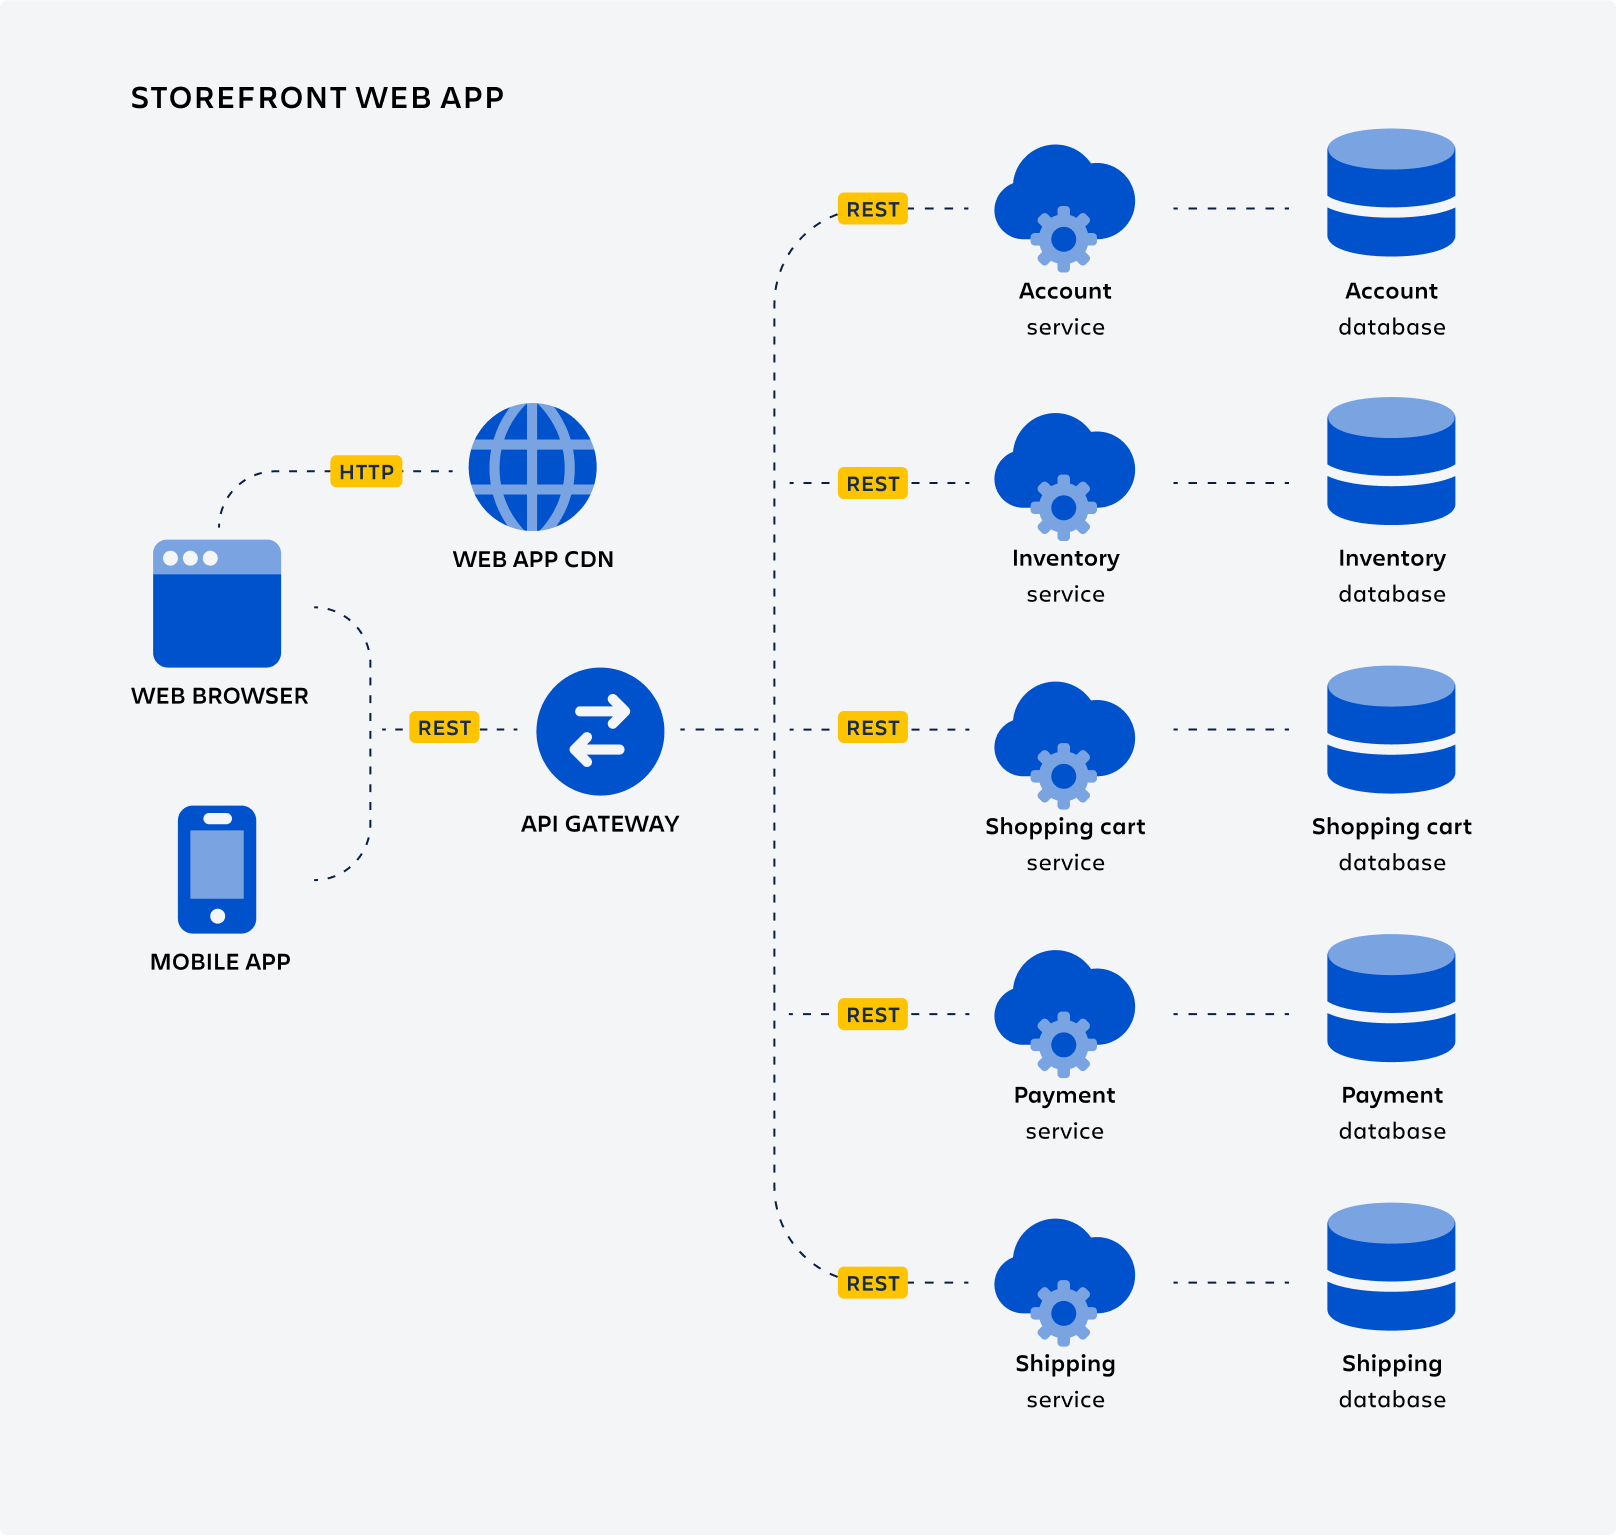
\includegraphics[width=0.3\textwidth]{figures/microservice.png}
    \end{center}
    \caption{Microservices architecture}
    \label{fig:2}
\end{figure}


\subsection{Kubernetes}

Kubernetes is a container-based platform that manages applications based on CPU, memory, or custom metrics. It is loosely coupled and extensible to meet different workloads.

Kubernetes is a platform for scheduling and running containers on clusters of physical or virtual machines (VMs). It helps you fully implement and rely on a container-based infrastructure in production environments. Developers can also create cloud-native apps with Kubernetes as a runtime platform by using Kubernetes patterns.

Kubernetes helps developers create multi-container applications by analyzing the configuration, finding resources appropriate for running the new containers, helping them connect to one another and to system resources, and monitoring the system for changes.


\subsubsection{Autoscaling}
The standard basis for autoscaling and scheduling in Kubernetes is resource utilization metrics.

\begin{figure}[!h]
    \begin{center}
        
\includegraphics[width=0.3\textwidth]{figures/kubernetes.png}
    \end{center}
    \caption{Kubernetes}
    \label{fig:Kubernetes}
\end{figure}

\subsection{Tracing}

Tracing is the specialized use of logging to record information about a program’s flow of execution.
Trace logs are used by programmers for debugging purposes, and by system administrators to diagnose common problems with software.

Several tools currently being used for tracing inside linux kernelspace. 

\subsubsection{ebpf}

eBPF is an advanced technology to run applications inside the kernel, but it is also heavier than purpose-built tracer like lttng

\subsection{Distributed Tracing}
                                                                                                                     Tracing the execution of a computer program is not a new concept, but modern architectures such as microservices have fundamentally broken the classic methods of profiling, debugging, and monitoring. Distributed tracing stands ready to fix these issues, but can be hard.
                                                                                                                     In a distributed system a daemon process running on a system can be measured in several dimensions, including the amount of memory mapped to the process. We can view open file handles, calculate CPU utilization, and do all sorts of things, but we can't trace the application.

\section{Motivation}
Microservices autoscaling in the cloud is directly linked with the cost of running the operation.

Many types of public and private Cloud systems require their users to declare how many instances their workload will need during execution, and the resources needed for each. Such limits make cloud computing possible, by enabling the Cloud infrastructure to provide adequate performance isolation. But limits are (mostly) a nuisance to the user.

\section{Related Work}

Some work has been done for enhancing the efficiency by utilizing ML and kernel tracing.

\subsection{Autopilot: workload autoscaling at google.\cite{b5}}

Google uses Autopilot to configure resources automatically, adjusting both the number of concurrent tasks in a job (horizontal scaling) and the CPU/memory limits for individual tasks (vertical scaling). Autopilot reduces slack by 23\% and the number of jobs severely impacted by OOMs by a factor of 10. Despite its advantages, ensuring that Autopilot was widely adopted took significant effort, including making potential recommendations easily visible to customers who had yet to opt in, automatically migrating certain categories of jobs, and adding support for custom recommenders.

\subsection{Firm}
This paper presents FIRM, an intelligent fine-grained resource management framework that uses online telemetry data and machine-learning methods to predictably share resources across microservices to drive up overall utilization. FIRM reduces service level objectives (SLOs) violations by up to 16 while reducing overall requested CPU limit by up to 62\%.

\subsection{Showar\cite{bShowar}}
SHOWAR shows a 22\% improvement with eBPF tracing.

\begin{figure}[!ht]
    \begin{center}
        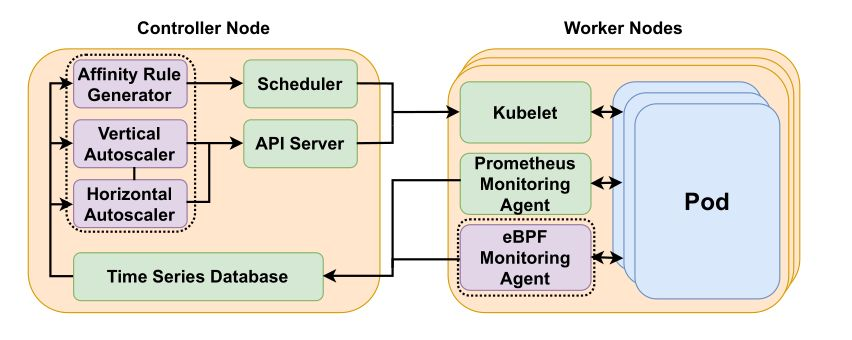
\includegraphics[width=0.45\textwidth]{figures/showar.png}
    \end{center}
    \caption{Showar Architecture}
    \label{fig:showar}
\end{figure}


\section{Experimentation}

\subsection{Showar\cite{bShowar} implementation}

As the authors implemented their implementation on DeathStarbench social-network microservice architecture, as a starting point of our project, we simulated their project and result.

\subsubsection{Detecting Run Queue Latency}

We introduced artificial load in linux server using 

\texttt{stress --cpu  1 --timeout 20}

Then we used eBPF to measure the run queue latency.

\texttt{runqlat 5 1}

It gave somewhat of a following graph:

\begin{figure}[!h]
    \begin{center}
        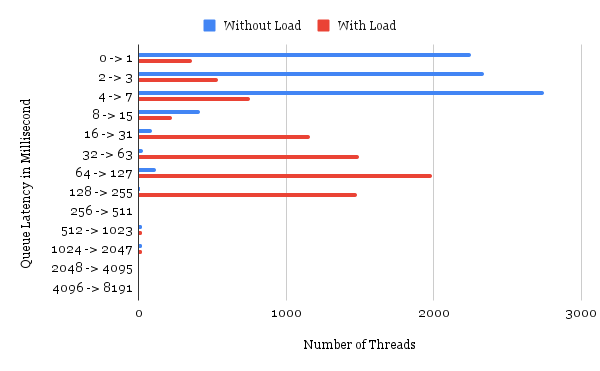
\includegraphics[width=0.45\textwidth]{figures/runqlat.png}
    \end{center}
    \caption{Histogram of queue latency comparing with artificial load given to the server}
    \label{fig:}
\end{figure}

The authors have used 95th quartile as the measure to autoscale kubernetes.

\subsection{System Setup}

For deploying our autoscaling algorithm developed using ebpf, we devised several ways:

\begin{enumerate}
    \item Deploying in a local machine.
        \begin{enumerate}
            \item Using Minikube (VirtualBox and Docker Driver)
            \item Using Apache Kind
        \end{enumerate}
    \item Deploying in Cloud environment.
        \begin{enumerate}
            \item In Cloud Vendors (AWS, Azure, GCP and DigitalOcean)
            \item In MetaCloud Frameworks (CloudLab)
        \end{enumerate}
\end{enumerate}


\begin{figure}[!h]
    \begin{center}
        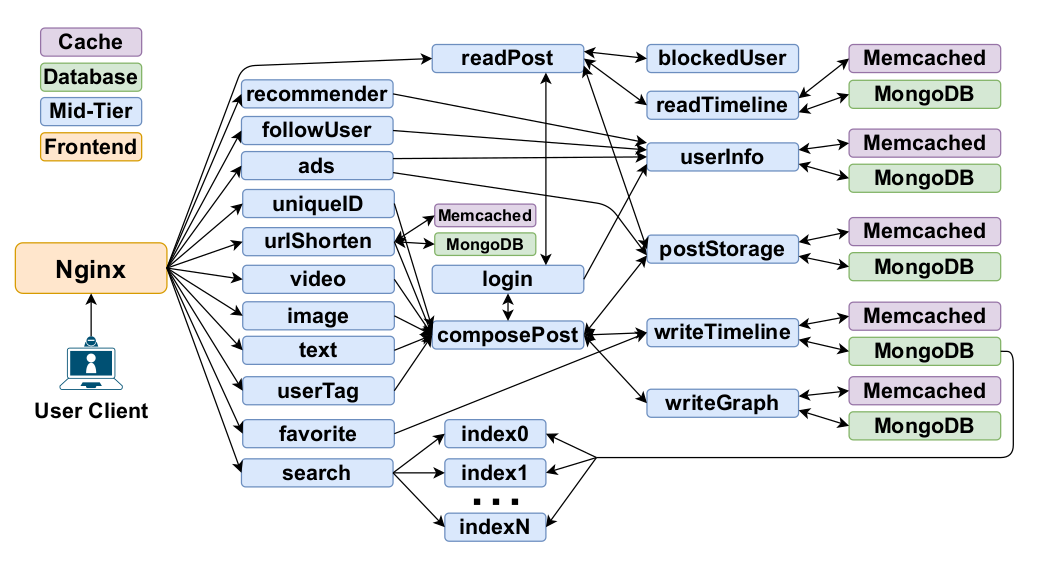
\includegraphics[width=0.4\textwidth]{figures/social-network.png}
    \end{center}
    \caption{DeathStarbench\cite{bDeathStarBench} Social Network application using microservices architecture}
    \label{fig:social-network}
\end{figure}


We were able to run the DeathStarbench framework in Local Machine. But, we were unable to run using Free instances of Cloud Vendors(AWS, Azure, GCP and DigitalOcean). Finally, we were able to run DeathStarbench using Cloudlab instances. We used 1 master node and 3 follower nodes in openstack \cite{bstack} configuration. Then we ran Microk8s (ubuntu specific Kubernetes framework) in them. 

\begin{figure}[!h]
    \begin{center}
        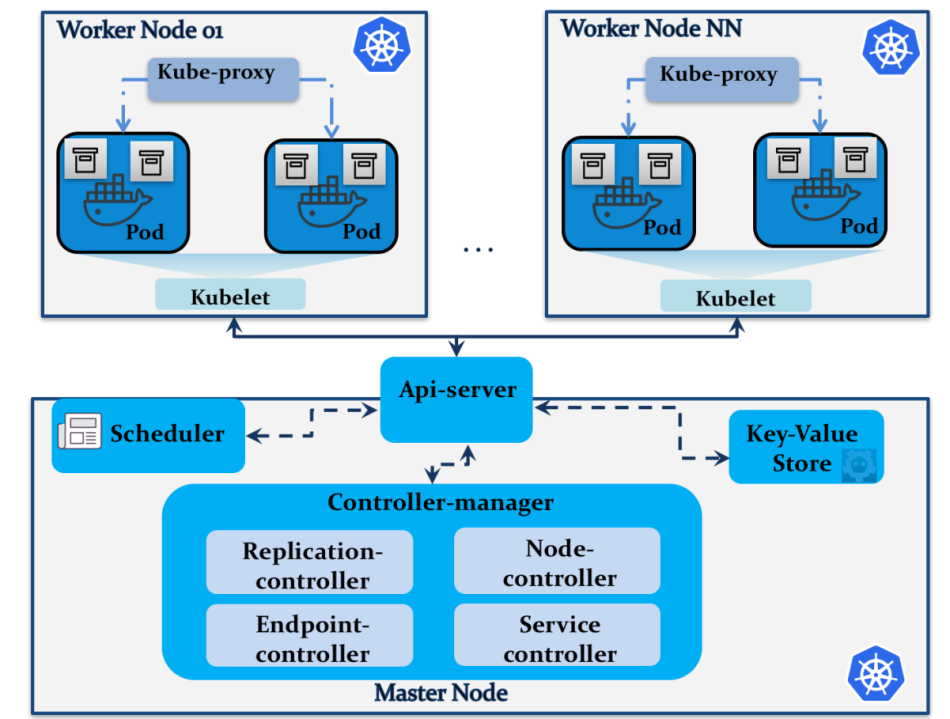
\includegraphics[width=0.45\textwidth]{figures/openstack-kube.png}
    \end{center}
    \caption{Kubernetes in cloudlab openstack}
    \label{fig:kube-cloudlab}
\end{figure}

\section{Future Work}

We were unable to setup a prometheus exporter for lack of time in the course. In the near future, we will try to implement a lTTng metrics exporter in cloudlab and gather microservice data and pass the data to Kubernetes autoscaler accordingly. 


\begin{thebibliography}{00}
    \bibitem{b54} Austin Parker, Daniel Spoonhower, Jonathan Mace, Ben Sigelman, and Rebecca Isaacs. 2020. Distributed tracing in practice: Instrumenting, analyzing, and debugging microservices. O’Reilly Media.
    \bibitem{bDeathStarBench} Yu Gan, Yanqi Zhang, Dailun Cheng, Ankitha Shetty, Priyal Rathi, Nayan Katarki, Ariana Bruno, Justin Hu, Brian Ritchken, Brendon Jackson, et al. 2019. An open-source benchmark suite for microservices and their hardware-software implications for cloud \& edge systems. In Proceedings of the Twenty-Fourth International Conference on Archi- tectural Support for Programming Languages and Operating Systems. 3–18.
    \bibitem{b3} \sloppy Martin Fowler. "Microservices". http://martinfowler.com/articles/\\microservices.html
    \bibitem{bShowar} Baarzi, Ataollah Fatahi, and George Kesidis. "Showar: Right-sizing and efficient scheduling of microservices." Proceedings of the ACM Symposium on Cloud Computing. 2021.
    \bibitem{b5} Rzadca, Krzysztof, et al. "Autopilot: workload autoscaling at google." Proceedings of the Fifteenth European Conference on Computer Systems. 2020.
    \bibitem{b6} 
    \bibitem{bebpf} Miano, Sebastiano, et al. "A framework for eBPF-based network functions in an era of microservices." IEEE Transactions on Network and Service Management 18.1 (2021): 133-151.
    \bibitem{bstack} Rosado, Tiago, and Jorge Bernardino. "An overview of openstack architecture." Proceedings of the 18th International Database Engineering \& Applications Symposium. 2014.
    \bibitem{netflix} \sloppy April, 01, 2021. Adopting microservices at Netflix. https://www.nginx.com/blog/microservices-at-netflix-architectural-best-practices/.
    \bibitem{azure} \sloppy April, 05, 2021. Microsoft Microservices Architecture Guide. https://docs.microsoft.com/enus/azure/architecture/guide/architecture-styles/microservices.
    \bibitem{google} \sloppy April, 10, 2021. Adapt or Die: A microservices story at Google, December. https://www.slideshare.net/apigee/adapt-or-die-a-microservicesstory-at-google.
    \bibitem{appEngine} \sloppy  April, 21, 2021. Microservices Architecture on Google App Engine. https://cloud.google.com/appengine/docs/standard/python/microserviceson-app-engine.
    \bibitem{burns} Brendan Burns. 2018. Designing Distributed Systems: Patterns and Paradigms for Scalable, Reliable Services. " O’Reilly Media, Inc.".
    \bibitem{wolff} Eberhard Wolff. 2016. Microservices: flexible software architecture. Addison-Wesley Professional.
    \bibitem{hao} Hao Zhou, Ming Chen, Qian Lin, Yong Wang, Xiaobin She, Sifan Liu, Rui Gu, Beng Chin Ooi, and Junfeng Yang. 2018. Overload control for scaling wechat microservices. In Proceedings of the ACM Symposium on Cloud Computing. 149–161.




    



\end{thebibliography}
\end{document}
